\documentclass[9pt, compress, xcolor=table]{beamer}


\usetheme{m}

\usepackage{amsmath,amssymb}
\usepackage{booktabs}
\usepackage[scale=2]{ccicons}
\usepackage{minted}
% \usepackage[utf8]{inputenc}
% \usepackage[T2A]{fontenc}
% \usepackage[english, russian]{babel}
%%% For accessing system, OTF and TTF fonts
%%% (would have been loaded by polylossia anyway)
\usepackage{fontspec}
%%% For language switching -- like babel, but for xelatex
\usepackage{polyglossia}
\setmainfont{PT Sans} % вообще шрифты определяются в теме бимера
\setmainlanguage{russian}
\setotherlanguages{english} %% or other languages

\usepackage{graphicx}
\usepackage{tabu} % https://ru.sharelatex.com/learn/Tables
\DeclareGraphicsExtensions{.pdf,.jpg,.png}
\graphicspath{{../images/}{./images/}}

\colorlet{Mycolor1}{green!50!blue!50!}

\usemintedstyle{trac}

\title{Физические принципы микроскопии сверхвысокого разрешения}
\subtitle{осенний семестр, 2018}
\author{ассистент, к.ф.-м.н. Шутова О.А.}
\institute{МГУ им. М.В. Ломоносова, физический факультет}

\begin{document}
\enablehyphenation

\maketitle

\plain{}{Лекция 3. Ближнее поле оптического зонда}

\begin{frame}{Идея лекции}

Ранее мы показали, что ближнее поле обладает рядом важных отличительных свойств по сравнению с плоской ЭМ волной или пучком в скалярном  приближении, такими как:
\begin{itemize}
\item наличие компоненты электрического поля вдоль направления распространения, т.н. продольное поле (т.е. оно направлено вдоль ОС системы)
\item сложное состояние поляризации
\item компоненты спектра, простирающиеся в закритическую область
\end{itemize}

Мы подчеркнули, что именно эти качества БП могут быть использованы для визуализации со сверхразрешением. Но следующим шагом на пути решения этой проблемы является задача \textcolor{red}{управления свойствами} ближнего поля. Рассмотрим три знакомые нам объекта: \textcolor{red}{линзу, апертуру и коническое острие} в области субволной оптики.

Но для начала посмотрим на \textcolor{red}{фотопортрет ближнего поля}, который в 2012 году был впервые получен с помощью GST-пленки немецкими учеными.

\end{frame}

\begin{frame}{Ближнее поле: фотопортрет}

\begin{center}
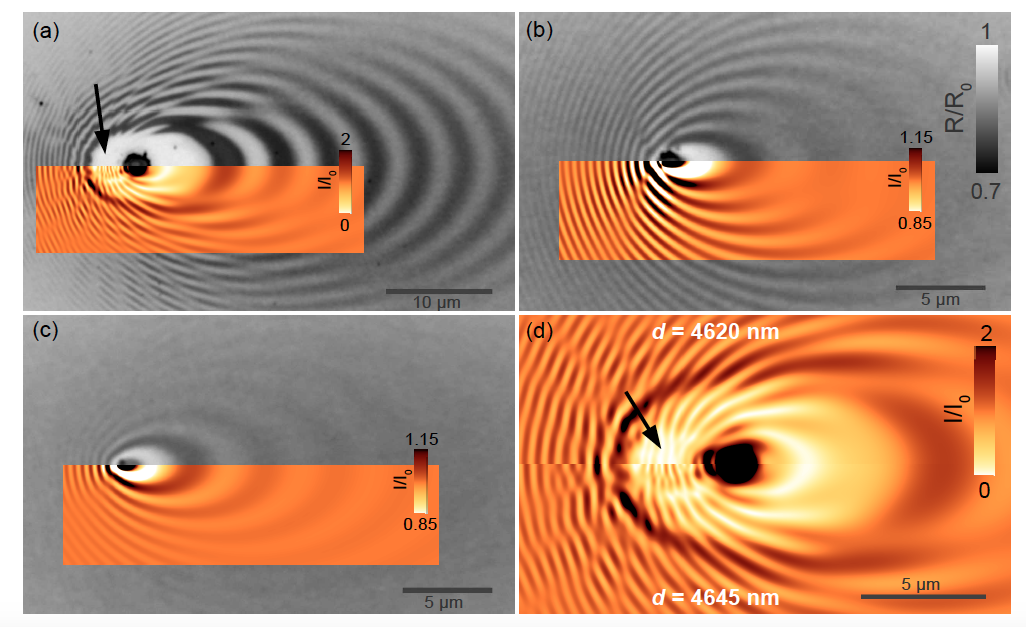
\includegraphics[width=0.8\textwidth]{near-field2}
\end{center}

С помощью аморфных пленок $Ge_2 Sb_5 Te_5$ (их еще обозначают GST-255), способных менять фазовое состояние под действием света (их применяют на современных носителях информации) можно записать картину распределения интенсивности БП.

\scriptsize{P. K\"uhler, "Quantitative imaging of optical near field", OPTICS EXPRESS. 2012. [1]}
\end{frame}

\begin{frame}{Свойства распределения}

\begin{center}
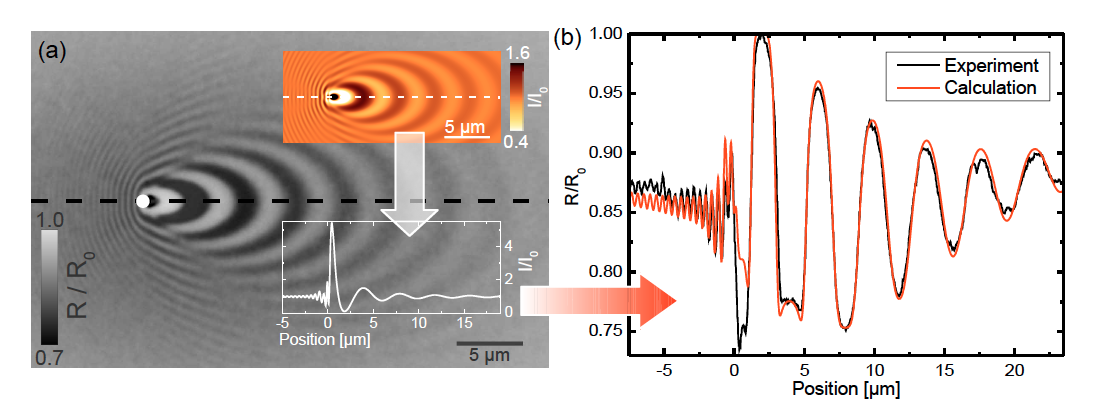
\includegraphics[width=0.95\textwidth]{near-field1}
\end{center}

Длина волны излучения $800$ нм, падает слева по углом $53^{0}$, диаметр кварцевой сферической частицы 1 микрон. Обратим внимание на то, что в картине распределения видны топографические сингулярности.

Для расчета ближнего поля вблизи диэлектрической сферической частицы, находящейся над плоской поверхностью, понадобится разложение в ряд по цилиндрическим функциям (см. Appendix в статье [1])
\end{frame}

\begin{frame}{Способы конструирования распределения поля}

\begin{itemize}
\item \textcolor{blue}{Малая диафрагма}: от подхода на основе интеграла Кирхгофа к теории Бете-Баукэмпа

\item \textcolor{blue}{Короткофокусная линза}: от геометрической оптики к решению Ричардса-Вольфа

\item \textcolor{blue}{Кольцевая диафрагма}: способ усилить продольное поле

\item \textcolor{blue}{Коническое острие}: от статического эффекта громоотвода к учету плазмонного резонанса

\item \textcolor{blue}{Управление поляризацией}: сложение разных мод, конструирование векторных пучков

\item \textcolor{blue}{Линейная БП микроскопия}: управляемая поляризация + отклик сигнала флуоресценции

\end{itemize}


\end{frame}

\begin{frame}{Решение Бете-Баукэмпа для малой диафрагмы}

Bethe-Bouwkamp solution

\begin{center}
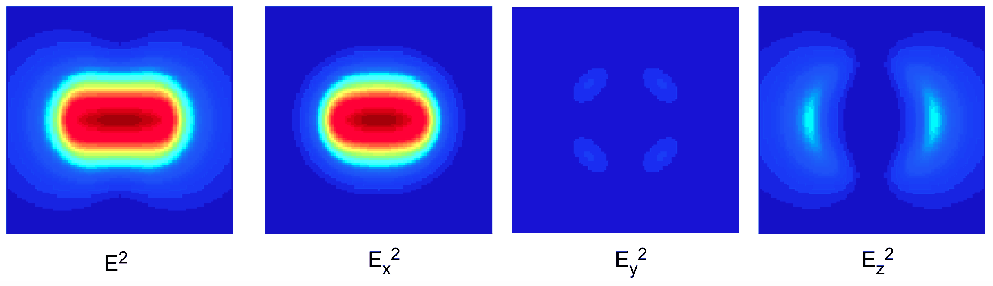
\includegraphics[width=0.9\textwidth]{bb}
\end{center}
Решение по теории Бете-Баукэмпа на расстоянии $z=0.3 a$, где $a$~--- диаметр отверстия, каждый рис.~--- область $4a*4a$.

Вдали от апертуры по мощности и угловому распределению теория Бете предсказывает распределение аналогичное полю двух диполей, электрического  и магнитного, сонаправленного соответствующим векторам падающей плоской волны, эффективно так бы рассеивала равновеликая сфера с восприимчивостью $\epsilon=2$. 

\end{frame}

\begin{frame}{Решение Бете-Баукэмпа для малой диафрагмы}
Пусть поле падает по нормали к экрану и поляризовано вдоль оси $x$, введем $\xi = \frac{a}{\rho}$, при этом $\rho$ и $\phi$~-- полярные координаты в плоскости диафрагмы, в плоскости апертуры ($z=0$):

\begin{equation*}
E_{\rho} = -E_0\frac{8\imath k_0 a}{3\pi}\frac{1-0.5\xi^2}{(1-\xi)^{1/2}}\cos \phi,
\end{equation*}
\begin{equation*}
E_{\phi} = E_0\frac{8\imath k_0 a}{3\pi}(1-\xi^2)^{1/2}\sin \phi,
\end{equation*}
\begin{equation*}
E_{z} = 0.
\end{equation*}

\underline{Свойства решения:}
\begin{itemize}
\item малая диафрагма пропускает значительно меньше света, чем можно ожидать, экстраполируя ф-лу Кирхгофа из чисто геометрических соображений. Сравним: $I=I_0 A_1(\theta) k^2a^4$ (К.) и $I=I_0 A_2(\theta) k^4a^6$ (Б.-Б. при $r\gg a$)
\item закон ``голубого цвета неба'' (рэлеевское рассеяние $I \propto \omega^4$): вырезает коротковолновую часть спектра
\item поляризация прошедшего поля не является линейной и остро зависит от поляризации падающего поля
\end{itemize}
\end{frame}


\begin{frame}{Гауссов пучок}

Введем параметры: $\rho^2 = x^2 + y^2$~--- ширина пучка и $z_0 = \frac{k w_0^2}{2}$~--- длина области перетяжки.

\begin{equation*}
\boxed{
\vec E(\rho,z) = \vec E_0 \frac{w_0}{w(z)}
\exp^{\frac{-\rho^2}{w(z)^2}}\exp^{\imath [kz - \eta(z) + k \rho^2/2R(z)]}}
\end{equation*}

\begin{equation*}
w(z) = w_0(1 + z^2/z_0^2)^{1/2}\text{~--- радиус пучка}
\end{equation*}

\begin{equation*}
R(z) = z(1 + z^2/z_0^2)\text{~--- радиус волнового фронта}
\end{equation*}

\begin{equation*}
\eta (z) = \arctan {z/z_0}\text{~--- фазовый сдвиг}
\end{equation*}
\textcolor{red}{Фазовый сдвиг Гюи}: сравнение с реперной плоской волной, сфазированной на $z \rightarrow -\infty$
дает расхождение на $z \rightarrow \infty$. Переход через перетяжку сдвигает фазу на $180^{\circ}$. Это означает, что даже в параксиальном приближении гауссов пучок ведет себя отлично от плоской волны.

\end{frame}


\begin{frame}{Продольные поля в фокальной области}
Пусть есть гауссов пучок, поляризованный вдоль оси $x$

\begin{equation*}
\boxed{
div\vec E = 0\hspace{0.5cm}\Longrightarrow\hspace{0.5 cm}E_z = - \int\left[\frac{\partial}{\partial x} E_x\right] dz}
\end{equation*} 

В плоскости перетяжки получим \begin{equation*} E_z(x,y,0) = -\imath \frac{2x}{kw_0^2} E_x(x,y,0)\end{equation*}

Итак, еще раз убеждаемся гауссов пучок не может быть плоской волной.

Мнимая единица указывает на сдвиг фазы на $90^{\circ}$. 

\textcolor{red}{Величина продольного поля зависит от того, насколько сильно мы ужали пучок.}

Это обстоятельство является для нас лишь \textcolor{red}{стартовой позицией}, потому что реально продольное поле гауссового пучка невелико, и концентрируется не там, где бы нам хотелось. Но разберемся, что будет если взять более высокие моды...

\end{frame}

\begin{frame}{Эрмитовы, лагерровы, тороидальные}

\textcolor{violet}{Мода Эрмита-Гаусса} $\vec E^{H}_{nm}$

\begin{equation*}
\vec E^H_{nm}(x,y,z) = w_0^{n+m}\frac{\partial^n}{\partial x^n}\frac{\partial^m}{\partial y^m}\vec E(x,y,z)
\end{equation*}

\textcolor{violet}{Мода Лагерра-Гаусса} $\vec E^{L}_{nm}$

\begin{equation*}
\vec E^L_{nm}(x,y,z) = k^n w_0^{2n+m} \exp^{\imath k z}\frac{\partial^n}{\partial z^n}
\left(\frac{\partial}{\partial x} + \frac{\partial}{\partial y}\right)^{m}\left(\vec E(x,y,z) \exp^{-\imath k z}\right)
\end{equation*}

\textcolor{violet}{Тороидальные (Doughnut) моды}

линейно-поляризованные: $\vec E^L_{01}$ и $\vec E^L_{11}$

Азимутально-поляризованные:  две перпендикулярно-поляризованные $\vec E^H_{01}$

Радиально-поляризованные: две перпендикулярно поляризованные $\vec E^H_{10}$

Лагерровы моды могут быть получены как суперпозиция конечного числа эрмитовых мод и наоборот.

\end{frame}

\begin{frame}{Сравнение продольных полей гауссовой и эрмитовой моды}

Иллюстрация наличия продольного поля для гауссова (слева) и эрмитова (справа) пучков.
\begin{columns}[c]
\column{6.5cm}
\begin{center}
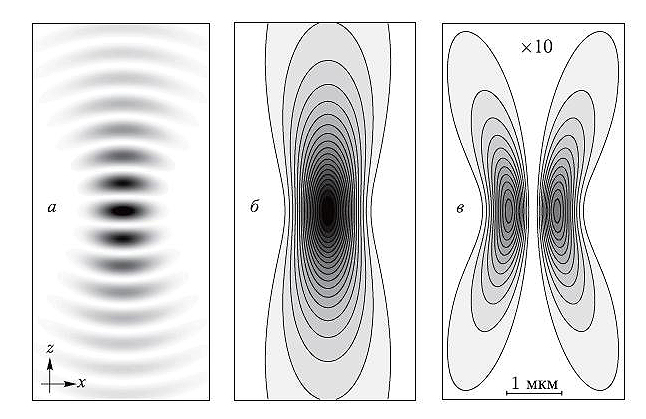
\includegraphics[width=5.5cm]{fig3_02}
\end{center}
\column{6.5cm}
\begin{center}
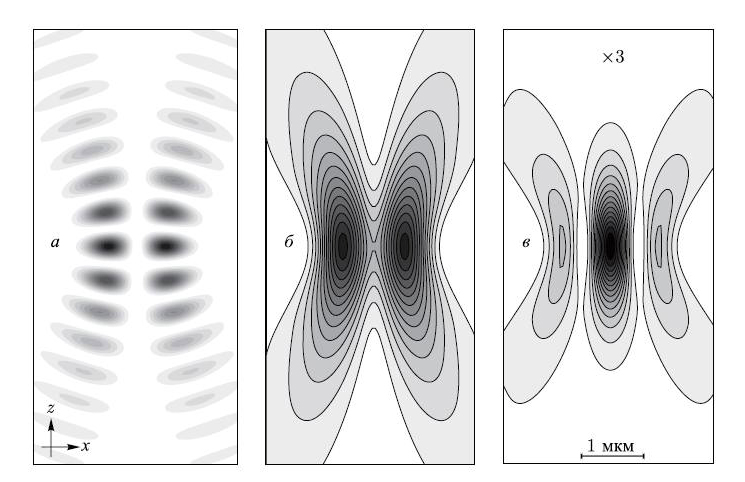
\includegraphics[width=5.5cm]{fig3_03}
\end{center}
\end{columns}
$\lambda=800$нм, $\theta = 28.65^{\circ}$

В центре ~--- полная интенсивность поля пучка. Справа ~--- интенсивность продольной компоненты.

Если мы будем смотреть на оптической оси, где поле больше всего интересует нас с точки зрения исследования, то  \textcolor{red}{гауссов пучок не имеет продольного поля на оси. У эрмитового, наоборот, там находится максимум.}
\end{frame}

\begin{frame}{Решение для поля, прошедшего через линзу}
Б.Ричардс, Э. Вольф (1959 г.) Electromagnetic diffration in optical systems. P.I. An integral representation of the image field. P. II. Structure of the image field in an aplanatic system. 

Рассмотрим фокусировку электромагнитной волны \textcolor{red!50!black}{короткофокусной (апланатической) линзой}. В этом случае мы не можем ограничится скалярным описанием процесса фокусировки:
\begin{multline*}
\vec E_{inc}^{(s)} = [\vec E_{inc} \cdot \vec n_{\phi}]\vec n_{\phi}\qquad
\vec E_{inc}^{(p)} = [\vec E_{inc} \cdot \vec n_{\rho}]\vec n_{\theta}\\
\vec E_{\infty} = \left[t^s [\vec E_{inc} \cdot \vec n_{\phi}]\vec n_{\phi} +
t^p [\vec E_{inc} \cdot \vec n_{\rho}]\vec n_{\theta}\right]\sqrt{\frac{n_1}{n_2}} (\cos \theta)^{1/2}.
\end{multline*}
\begin{multline*}
\vec E_{\infty}(\theta, \phi) = t^s(\theta) \left[ \vec E_{inc}(\theta, \phi)\cdot
\left(\array{c} -\sin \theta
\\ \cos \phi \\ 0 \endarray\right)\right] \left(\array{c}
-\sin \phi \\ \cos \phi \\ 0 \endarray\right) \sqrt{\frac{n_1}{n_2}} (\cos \theta)^{1/2} +
\\ + t^p(\theta) \left[ \vec E_{inc}(\theta, \phi) \cdot \left(\array{c} \cos \phi \\ \sin \phi \\ 0
\endarray\right)\right] \left(\array{c} \cos \phi \cos \theta \\ \sin \phi \cos \theta \\ -\sin \theta \endarray\right)
\sqrt{\frac{n_1}{n_2}} (\cos \theta)^{1/2},
\end{multline*}

\scriptsize{См. по Л. Новотный, Б. Хехт "Основы нанооптики", гл. 4.}
\end{frame}

\begin{frame}{Перепишем выражение для поля в дальней зоне}

для линзы с антибликовым покрытием $\vec E_{inc} = E_{inc} \vec n_x$; $t_{\theta}^s =
t_{\theta}^p = 1$

\begin{multline*}
\vec E_{\infty}(\theta, \phi) =E_{\infty}(\theta,\phi)[\cos \phi \vec n_{\theta} - \sin \phi\vec
n_{\phi}] \sqrt{\frac{n_1}{n_2}} =
\\ =E_{\infty}(\theta, \phi) \frac{1}{2}\left[\array{c} (1 +
\cos \theta) - (1 - \cos \theta) \cos 2 \phi \\ - (1 - \cos \theta) \sin 2 \phi \\ - 2 \cos \theta
\sin \phi
\endarray\right] \sqrt{\frac{n_1}{n_2}} (\cos \theta)^{1/2},
\end{multline*}

(0,0):$ E_{inc} = E_0 \exp^{(-x_{\infty}^2 + y_{\infty}^2)/ w_0^2} = E_0 \exp^{-f^2 \sin^2 \theta
/ w_0^2}$

\medskip

(1,0):$ E_{inc} = E_0 \frac{2 x_{\infty}}{w_0}\exp^{-(x_{\infty}^2 + y_{\infty}^2)/w_0^2} = \frac{2
E_0 f}{w_0} \sin \theta \cos \phi \exp^{-f^2 \sin^2 \theta / w_0^2}$

\medskip

(0,1):$ E_{inc} = E_0 \frac{2 y_{\infty}}{w_0}\exp^{-(x_{\infty}^2 + y_{\infty}^2)/w_0^2} = \frac{2
E_0 f}{w_0} \sin \theta \sin \phi \exp^{-f^2 \sin^2 \theta / w_0^2}$


\end{frame}

\begin{frame}{Функция аподизации}

Диафрагмальный радиус: $f \sin \theta_{max}$, фактор перекрытия $f_0 = \frac{w_0}{f \sin
\theta_{max}}$

Функция аподизации:

\begin{equation*}
f_w(\theta) = \exp^{-\frac{1}{f_0^2}\frac{\sin^2 \theta}{\sin^2 \theta_{max}}}.
\end{equation*}

\begin{center}
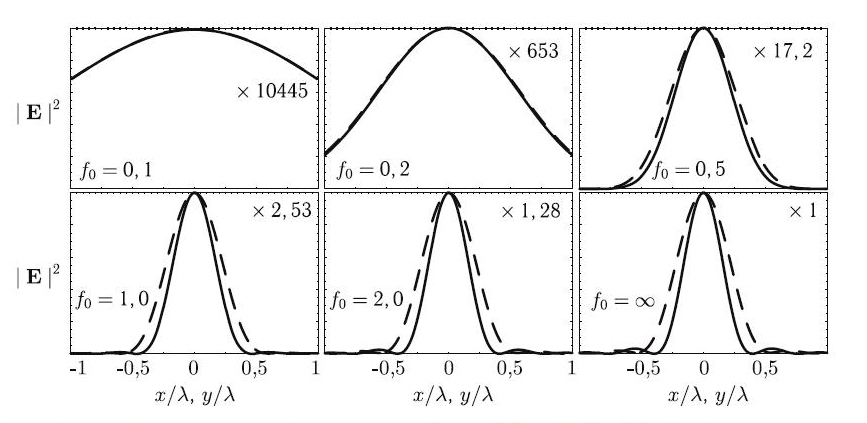
\includegraphics[width=9cm]{fig3_07}
\end{center}

\small{Влияние фактора перекрытия $f_0$ выходной диафрагмы на ширину фокуса. $NA = 1.4$, $n=1.518$, $|\vec E|^2$ показано в фокальной плоскости $z = 0$, пунктирные кривые вычислены вдоль оси $x$, а сплошные вдоль оси $y$.}


\end{frame}

\begin{frame}{Интегралы}

\begin{equation*}
I_{00} = \int_{0}^{\theta_{max}} f_w (\theta) (\cos \theta)^{1/2} \sin \theta (1+ \cos \theta) J_0(k \rho \sin \theta)
\exp^{\imath k z \cos \theta} d \theta
\end{equation*}

\begin{equation*}
I_{01} = \int_{0}^{\theta_{max}} f_w (\theta) (\cos \theta)^{1/2} \sin^2 \theta J_1(k \rho \sin \theta)
\exp^{\imath k z \cos \theta} d \theta
\end{equation*}

\begin{equation*}
I_{02} = \int_{0}^{\theta_{max}} f_w (\theta) (\cos \theta)^{1/2} \sin \theta (1- \cos \theta) J_2(k \rho \sin \theta)
\exp^{\imath k z \cos \theta} d \theta
\end{equation*}

\begin{equation*}
I_{10} = \int_{0}^{\theta_{max}} f_w (\theta) (\cos \theta)^{1/2} \sin^3 \theta J_0(k \rho \sin \theta)
\exp^{\imath k z \cos \theta} d \theta
\end{equation*}

\begin{equation*}
I_{11} = \int_{0}^{\theta_{max}} f_w (\theta) (\cos \theta)^{1/2} \sin^2 \theta (1 + 3 \cos \theta) J_1(k \rho \sin \theta)
\exp^{\imath k z \cos \theta} d \theta
\end{equation*}

\begin{equation*}
I_{12} = \int_{0}^{\theta_{max}} f_w (\theta) (\cos \theta)^{1/2} \sin^2 \theta (1- \cos \theta) J_1(k \rho \sin \theta)
\exp^{\imath k z \cos \theta} d \theta
\end{equation*}

\end{frame}


\begin{frame}{Решения Ричардса-Вольфа для ЭМ}

(0,0)-мода:\begin{equation*}
\begin{gathered}
\vec E(\rho, \theta, z) = \frac{\imath k f}{2} \sqrt {\frac{n_1}{n_2}}E_0 e^{-\imath k f}
\left[\array{c} I_{00} + I_{02}\cos 2 \phi \\ I_{02} \sin 2 \phi \\ -2 \imath I_{01}\cos \phi
\endarray\right] (\cos \theta)^{1/2}
\end{gathered}
\end{equation*}


(1,0)-мода:\begin{equation*}
\begin{gathered}
\vec E(\rho, \theta, z) = \frac{\imath k f^2}{2w_0} \sqrt {\frac{n_1}{n_2}}E_0 e^{-\imath k f}
\left[\array{c} \imath I_{11} \cos \phi + \imath I_{14}\cos 3 \phi \\ - \imath I_{12} \sin \phi +
\imath I_{14}\sin 3\phi
 \\ 2 I_{10} + 2 I_{13}\cos 2 \phi \endarray\right]
(\cos \theta)^{1/2}
\end{gathered}
\end{equation*}

(0,1)-мода:\begin{equation*}
\begin{gathered}
\vec E(\rho, \theta, z) = \frac{\imath k f^2}{2w_0} \sqrt {\frac{n_1}{n_2}}E_0 e^{-\imath k f}
\left[\array{c} \imath (I_{11} + 2I_{12}) \sin \phi + \imath I_{14}\sin 3 \phi \\ - \imath I_{12}
\cos \phi - \imath I_{14}\cos 3\phi
 \\ 2 I_{13}\sin 2 \phi \endarray\right]
(\cos \theta)^{1/2}
\end{gathered}
\end{equation*}

\end{frame}

\begin{frame}{Радиально- и азимутально-поляризованные пучки}

Радиально-поляризованная тороидальная мода:

\begin{equation*}
RP = HG_{10} \vec n_x + HG_{10}\vec n_y,
\end{equation*}

Азимутально-поляризованная тороидальная мода:

\begin{equation*}
AP = - HG_{01} \vec n_x + HG_{01} \vec n_y.
\end{equation*}

\begin{columns}[c]
\column{6cm}

\begin{center}
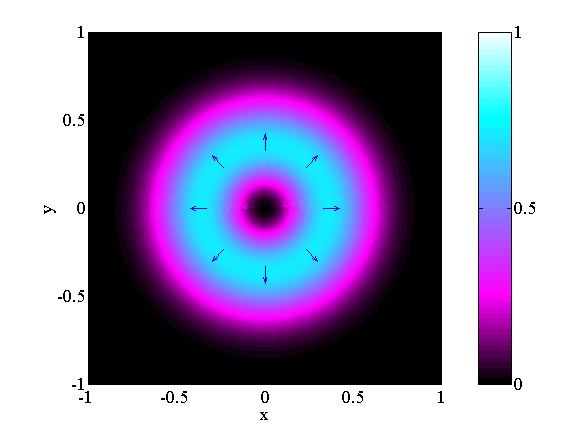
\includegraphics[width=5cm]{fig3_13}
\end{center}

\column{6cm}
\begin{center}
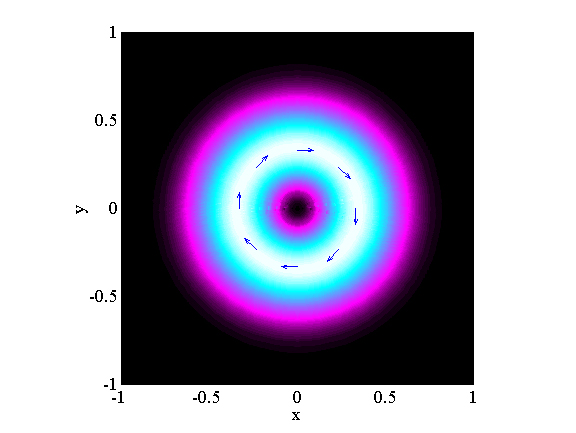
\includegraphics[width=5cm]{fig3_17}
\end{center}
\end{columns}


\end{frame}

\begin{frame}{Векторная запись радиально- и азимутально-поляризованного поля}

RL:
\begin{equation*}
\begin{gathered}
\vec E = -\frac{\imath E_0}{\pi}\int \limits_0^{\alpha}\int \limits_0^{2 \pi}g(\theta, \phi)
\left[\array{c} \cos \theta \cos \phi \\ \cos \theta \sin \phi \\ \sin \theta \endarray\right]d\theta d\phi
\end{gathered}
\end{equation*}

$E_z \neq 0, E_{\rho} \neq 0, E_{\phi} = 0$

\medskip

AL:
\begin{equation*}
\begin{gathered}
\vec E = -\frac{\imath E_0}{\pi}\int \limits_0^{\alpha}\int \limits_0^{2 \pi}g(\theta, \phi)
\left[\array{c} - \sin \phi \\ \cos \phi \\ 0 \endarray\right]d\theta d\phi
\end{gathered}
\end{equation*}

$E_z = 0, E_{\rho} = 0, E_{\phi} \neq 0$

\begin{block}{Линейно-поляризованная тороидальная мода: }
\begin{equation*}
RP = HG_{10} \vec n_x + \imath HG_{01}\vec n_y,
\end{equation*}
\end{block}

\end{frame}


\begin{frame}{Решения Ричардса-Вольфа для тороидальных мод}

Радиально-поляризованная тороидальная мода:

\begin{equation*}
\begin{gathered}
\vec E(\rho, \varphi, z) = \frac{\imath k f^2}{2w_0} \sqrt
{\frac{n_1}{n_2}}E_0 e^{-\imath k f} \left[\array{c} \imath
(I_{11}-I_{12}) \cos \varphi \\  \imath (I_{11}-I_{12}) \sin
\varphi \\ -4 I_{10} \endarray\right]
\end{gathered}
\end{equation*}

Азимутально-поляризованная тороидальная мода:

\begin{equation*}
\begin{gathered}
\vec E(\rho, \varphi, z) = \frac{\imath k f^2}{2w_0} \sqrt
{\frac{n_1}{n_2}}E_0 e^{-\imath k f} \left[\array{c} \imath
(I_{11}+3 I_{12}) \sin \varphi \\ - \imath (I_{11}+ 3 I_{12})
\cos \varphi \\ 0 \endarray\right]
\end{gathered}
\end{equation*}
Итак, радиально-поляризованная мода позволяет получить максимальное продольное поле: зависимость от NA
\begin{center}
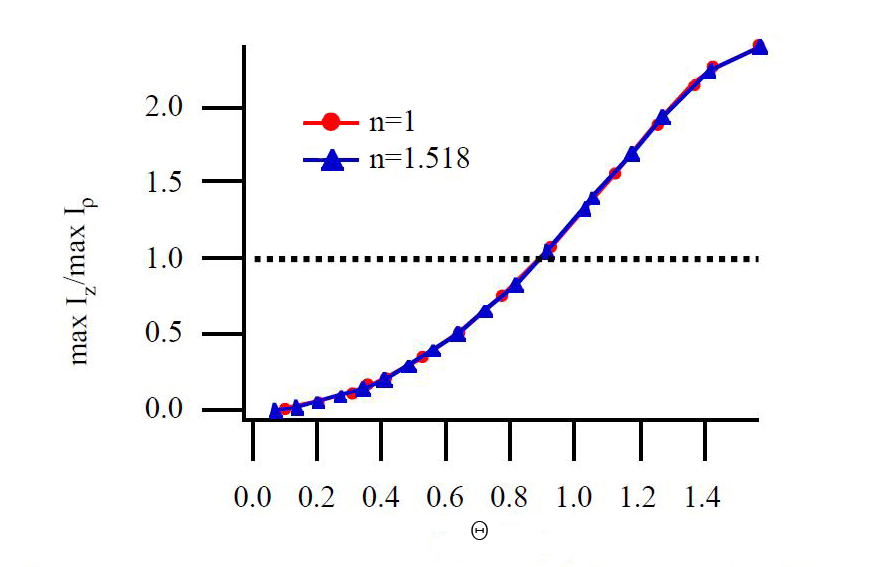
\includegraphics[width=5cm]{fig3_19}
\end{center}

\end{frame}

\begin{frame}{Циркулярно-поляризованное поле}
    
Можно составить циркулярно-поляризованное поле канонически из двух линейно-поляризованных вдоль x и y
полей, сдвинутых по фазе на величину, кратную нечетному числу $\pi/2$:

\begin{equation*}
\begin{gathered}
\vec E(\rho, \theta, z)_{\pm} = \frac{\imath k f}{2} \sqrt {\frac{n_1}{n_2}}E_0 e^{-\imath k f}
\left[\array{c} I_{00} + I_{02}\cos 2 \phi \pm \imath I_{02} \sin 2 \phi\\ I_{02} \sin 2 \phi \pm I_{00} + I_{02}\cos 2 \phi\\ -2 \imath I_{01}(\cos \phi\pm\imath \sin\phi)
\endarray\right] (\cos \theta)^{1/2}
\end{gathered}
\end{equation*}
Где $\pm$ означает вращение в одну и другую сторону (т.н. спиральность, helicity).

\textcolor{red!50!black}{Однако}, в этом случае средняя по периоду компонента поля в продольном направлении будет равна нулю.

Если наша задача стоит так, что нам необходимо уметь различить хиральность вещества (что особенно важно при исследовании биомолекул), такое поле не подойдет для исследования.
    
\end{frame}


\begin{frame}{Гибридное состояние поляризации}
    
\small{Чтобы решить эту проблему вводят гибридное состояние поляризации (HR) и циркулярно-поляризованное гибридное состояние поляризации (CPHR), являющееся суперпозицией радиально- и азимутально-поляризованных полей с задержкой по фазе и без:}
    \begin{columns}[c]
\column{7cm}
\begin{multline*}
\begin{gathered}
\vec E(\rho, \varphi, z)_{\pm}^{(CP)HR} = \frac{\imath k f^2}{2w_0} \sqrt
{\frac{n_1}{n_2}}E_0 e^{-\imath k f} \times\\\times \left[\array{c} 
(I_{11}-I_{12}) \cos \varphi \pm  (\imath)
(I_{11}+3 I_{12}) \sin \varphi \\  \imath (I_{11}-I_{12}) \sin
\varphi \mp (imath) (I_{11}+ 3 I_{12})
\cos \varphi\\ 4 \imath I_{10} \endarray\right]
\end{gathered}
\end{multline*}
\begin{enumerate}
  \small{  \item Если ввести нулевую фазовую задержку, мы получим линейную поляризацию, но изменяющую наклон в зависимости от азимутального угла.
    \item Если задержка равна $\pi/2$, получается циркулярно-поляризованная гибридная мода.
    \item Знак $\pm$ определяется спиральностью падающего поля. Мнимая единица в скобках появляется только при CPHR.}
\end{enumerate}
\column{5.5cm}
\begin{center}
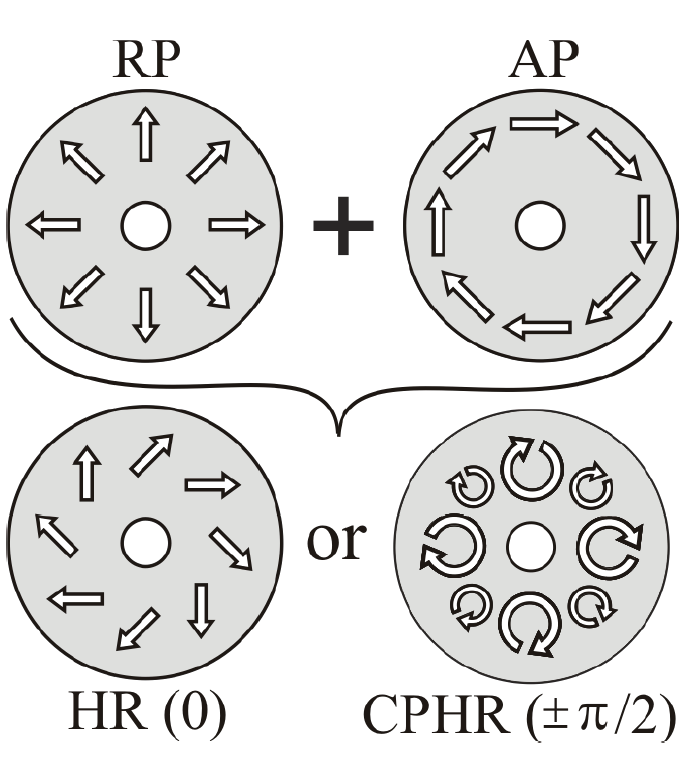
\includegraphics[width=0.9\textwidth]{hybrid}
 \end{center}
 
\end{columns}
    
\end{frame}

\begin{frame}{Электростатическое решение задачи о тонком коническом острие}
\begin{columns}[c]
\column{4cm}
\begin{center}
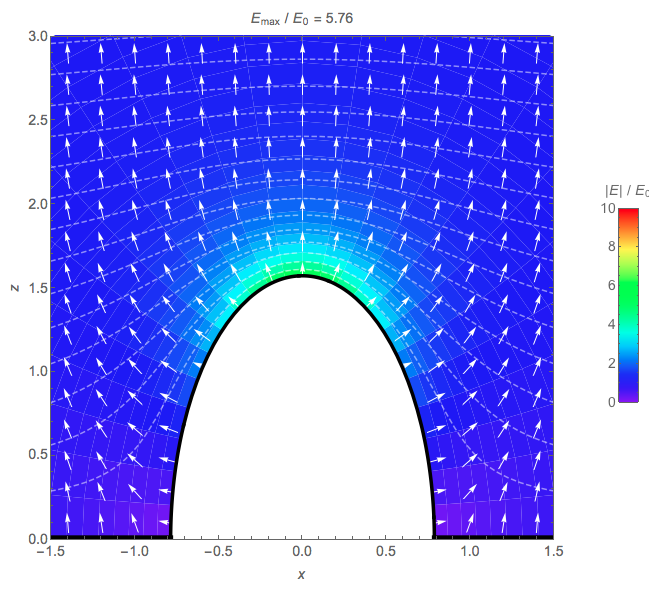
\includegraphics[width=\textwidth]{stat3}
 \end{center}
\column{4cm}
\begin{center}
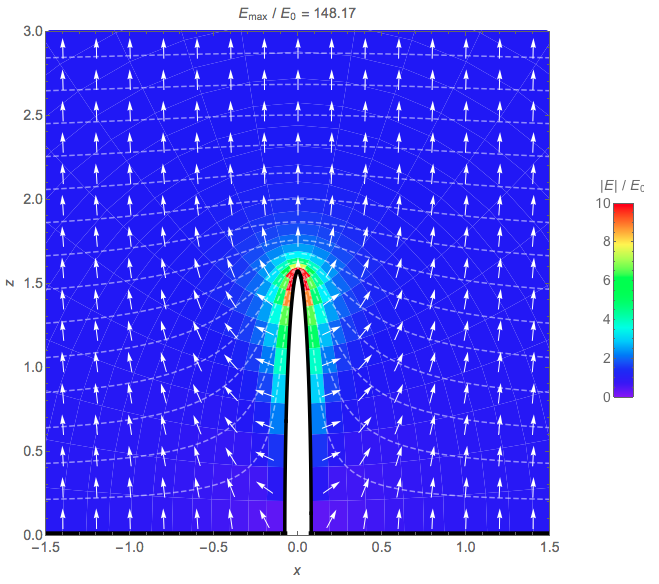
\includegraphics[width=\textwidth]{stat1}
 \end{center}
 \column{4cm}
\begin{center}
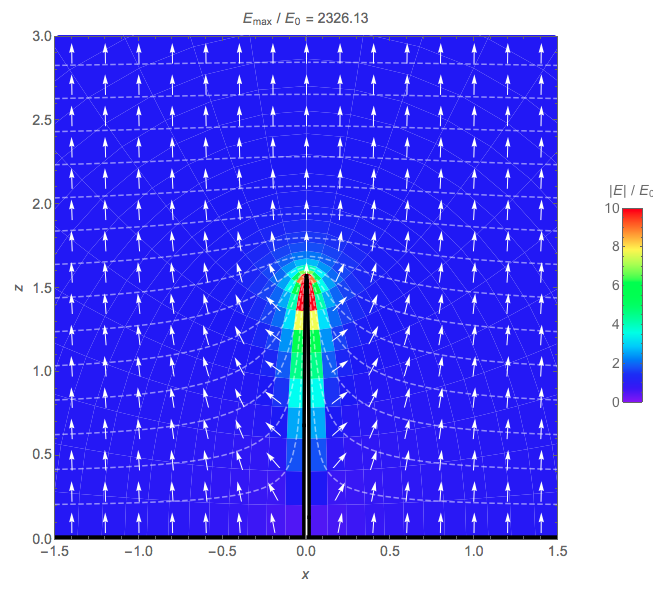
\includegraphics[width=\textwidth]{stat2}
\end{center}
\end{columns}

Ландау, Лифшиц, "<Электродинамика сплошных сред">, т.VIII, 1992, с. 33 или А. Стреттон, "<Теория электромагнетизма">

\begin{equation*}
\varphi = \varphi_0 + \varphi_1 = -a E_0 \cosh\xi\cos\eta\left(1-{\int_\xi^\infty d\xi \sinh^{-1}\xi\cosh^{-2}\xi}/{\int_{\xi_0}^\infty d\xi \sinh^{-1}\xi\cosh^{-2}\xi}\right)
\end{equation*}

\end{frame}

\begin{frame}{Электродинамическое решение задачи о тонком коническом острие}
Рассмотрим металлический эллипсоид с осями $a$ и $b$, меньшими длины волны излучения (чтобы пренебречь запаздыванием потенциала), и диэлектрической проницаемостью по теории Друде $\epsilon \approx 1+\frac{\omega_p^2}{\imath\gamma\omega -\omega^2}=\epsilon'+\imath \epsilon"$, тогда поле у вершины будет иметь вид:

\begin{equation*}
\vec E = \epsilon \vec E_0\frac{1}{1+A(a,b)(1-\epsilon)}
\end{equation*}

$A(a,b)$ - деполяризационный форм-фактор, который при достаточной вытянутости нашего эллипсоида ($a>>b$) будет иметь вид:

\begin{equation*}
A(a,b) = \left(\frac{b}{a}\right)^2 ln \frac{b}{a}
\end{equation*}

\begin{columns}
\column{8cm}
\begin{centering}
\begin{equation*}\boxed{
\omega_{res}=\sqrt{A(a,b)\omega_p^2-\gamma^2}}
\end{equation*}

\begin{equation*}
\boxed{\vec E = -\imath \frac{\epsilon \vec E_0}{\epsilon"(\omega_{res}) A(a,b)} \approx\frac{1}{A(a,b)}\left(1+\imath\frac{\omega_{res}}{\gamma}\right)}
\end{equation*}
\end{centering}
\column{4cm}
При соотношении осей $a/b=10$ в серебре можно достичь увеличения интенсивности на 3 порядка
\end{columns}
\end{frame}

\begin{frame}{Обобщение теории рассеяния Ми на эллипсоидальные формы (Ми-Ганса)}

\begin{center}
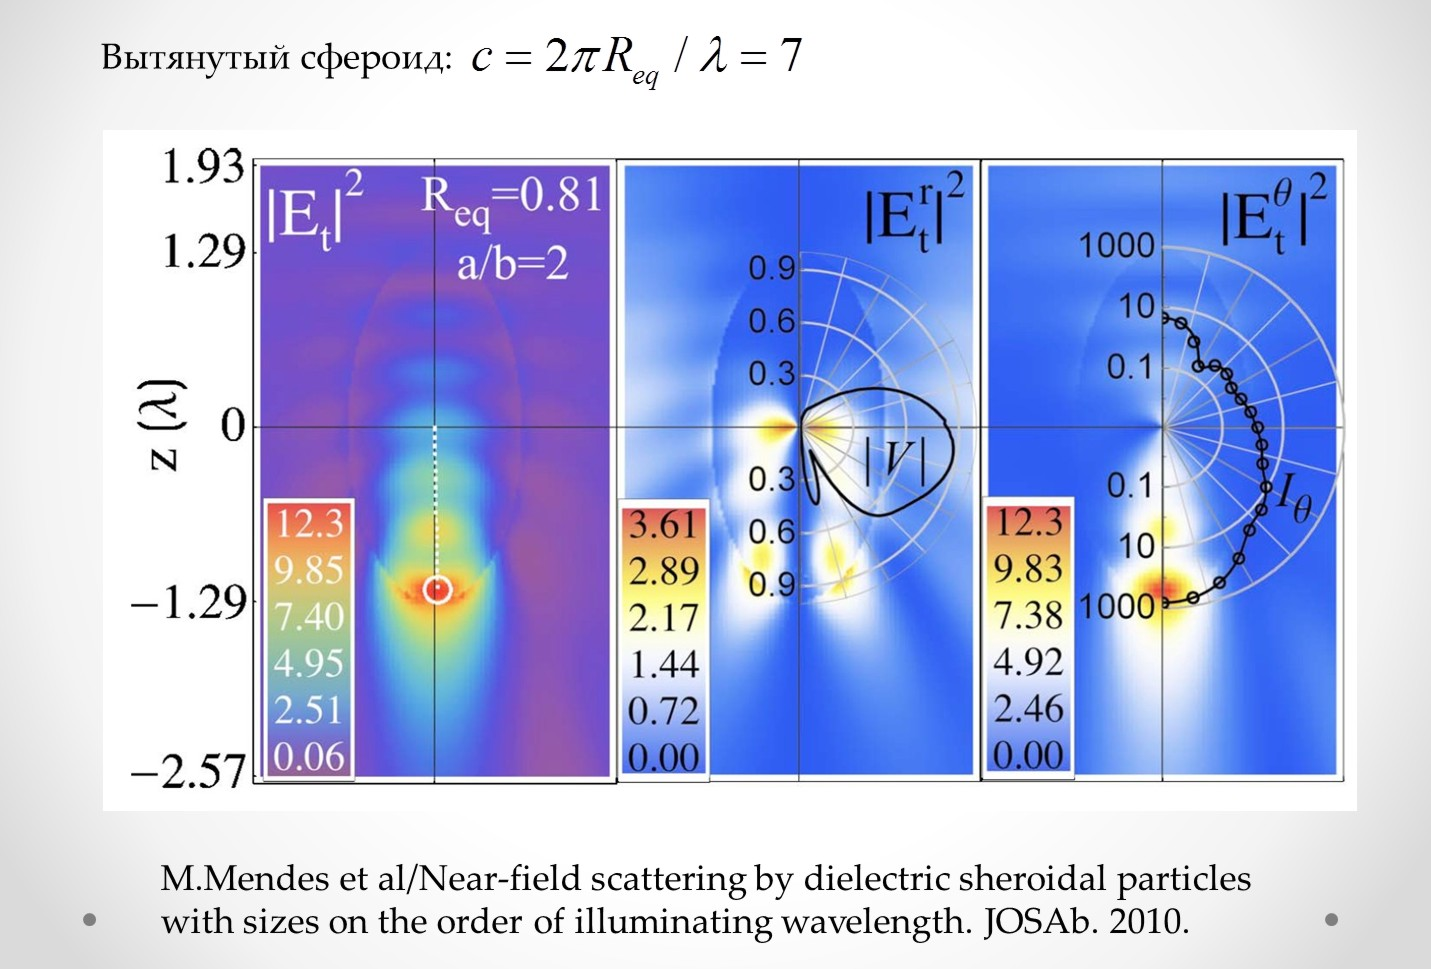
\includegraphics[width=\textwidth]{add_sl1}
\end{center}
\end{frame}


\begin{frame}{Обобщение теории рассеяния Ми на эллипсоидальные формы (Ми-Ганса)}
    
\begin{center}
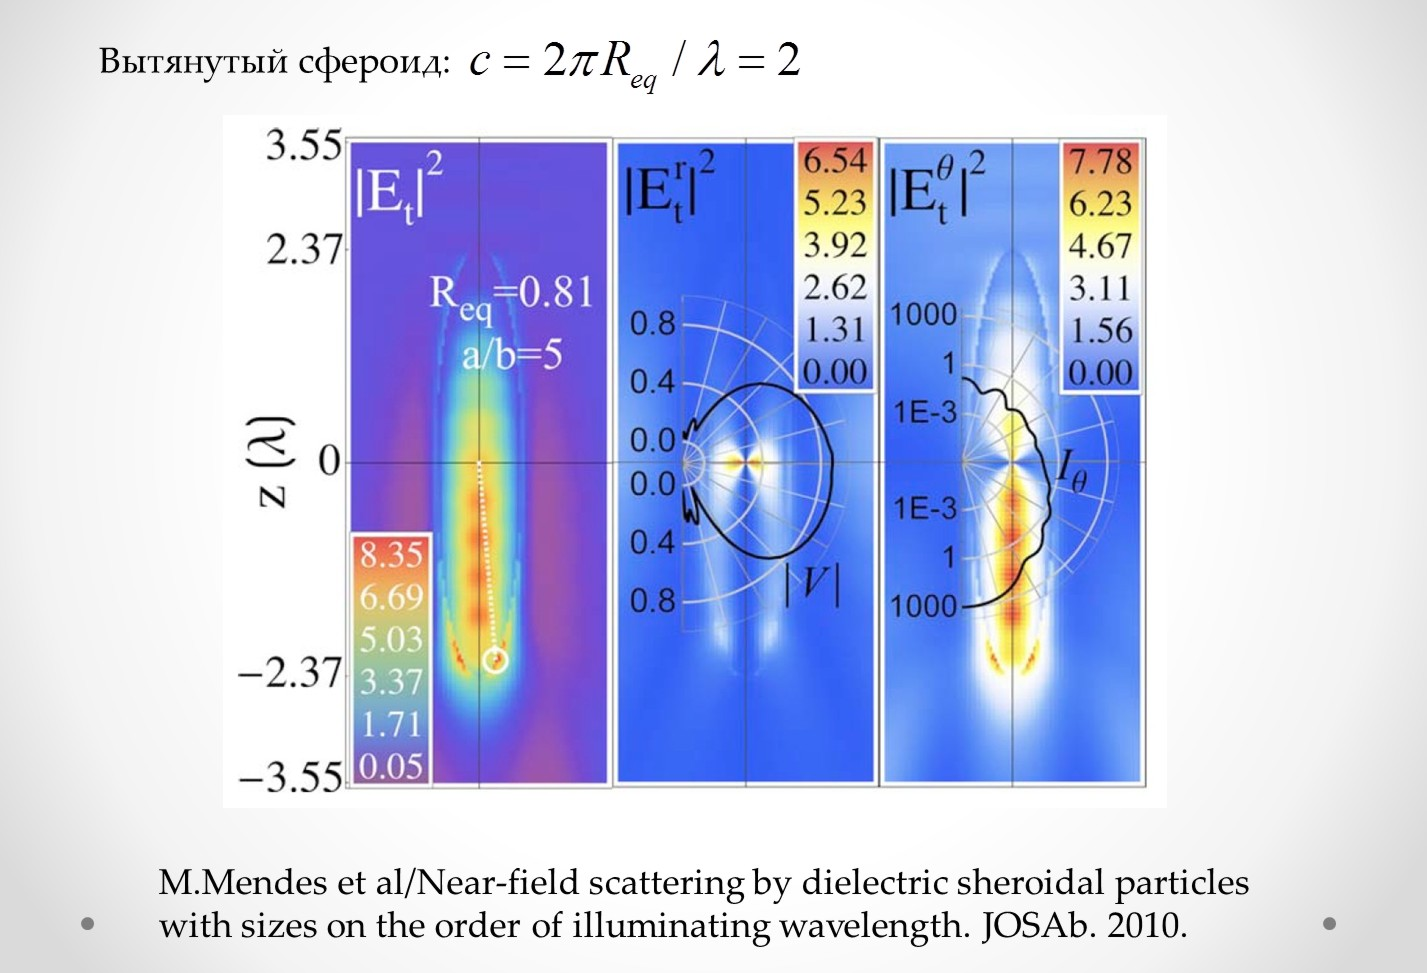
\includegraphics[width=1.1\textwidth]{add_sl2}
\end{center}
\end{frame}

\begin{frame}{Обобщение теории рассеяния Ми на эллипсоидальные формы (Ми-Ганса)}

\begin{center}
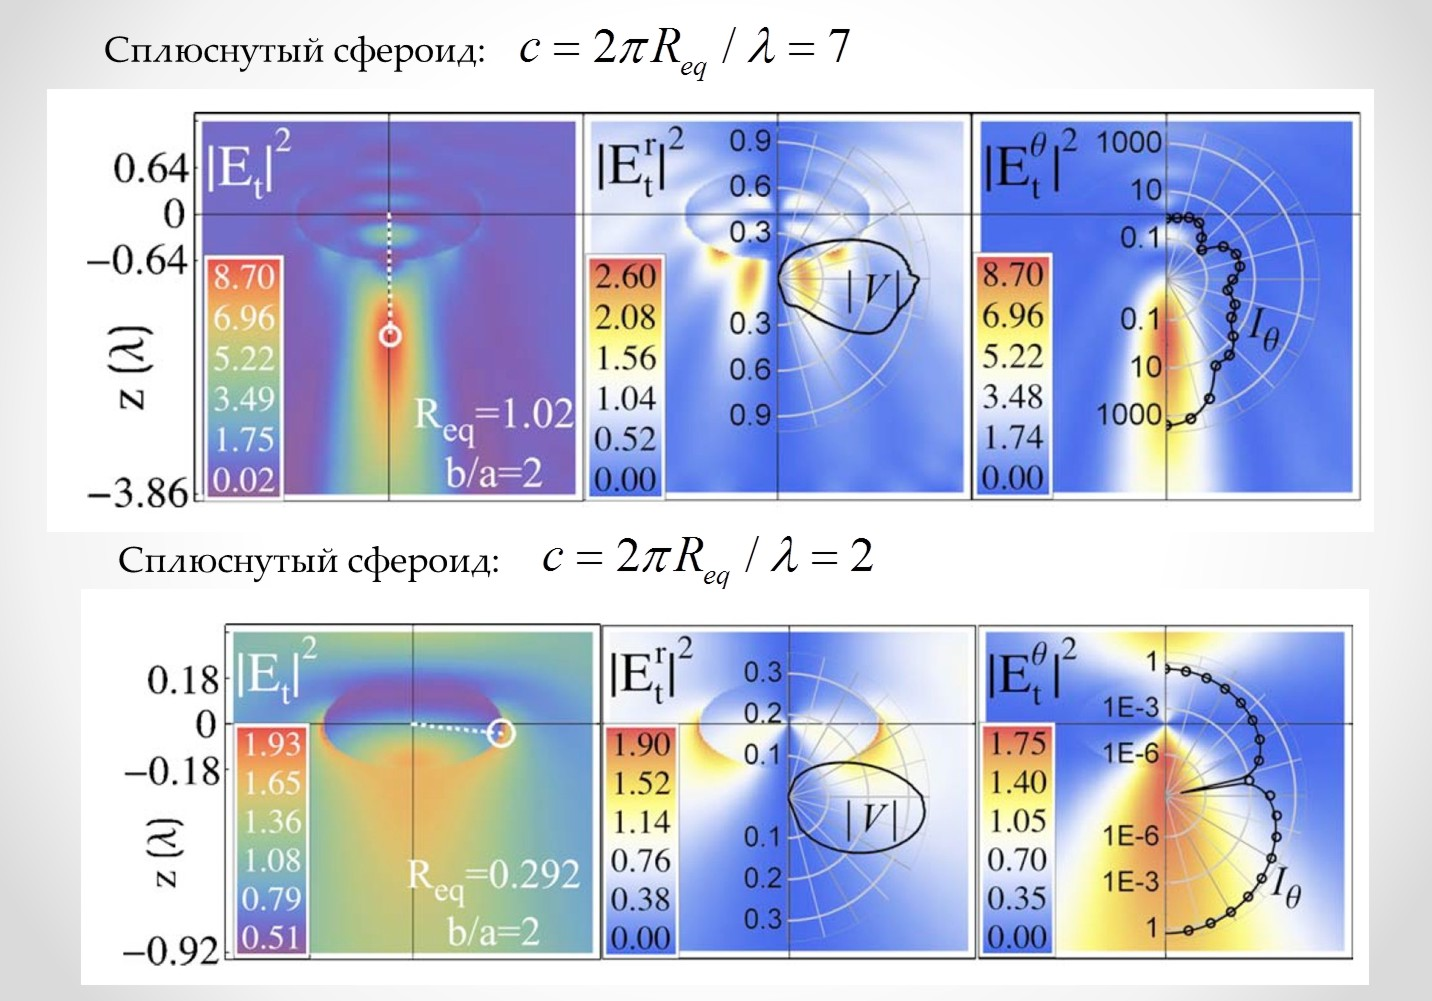
\includegraphics[width=1.1\textwidth]{add_sl3}
\end{center}
    
\end{frame}

\begin{frame}{Обобщение теории рассеяния Ми на эллипсоидальные формы (Ми-Ганса)}

\begin{center}
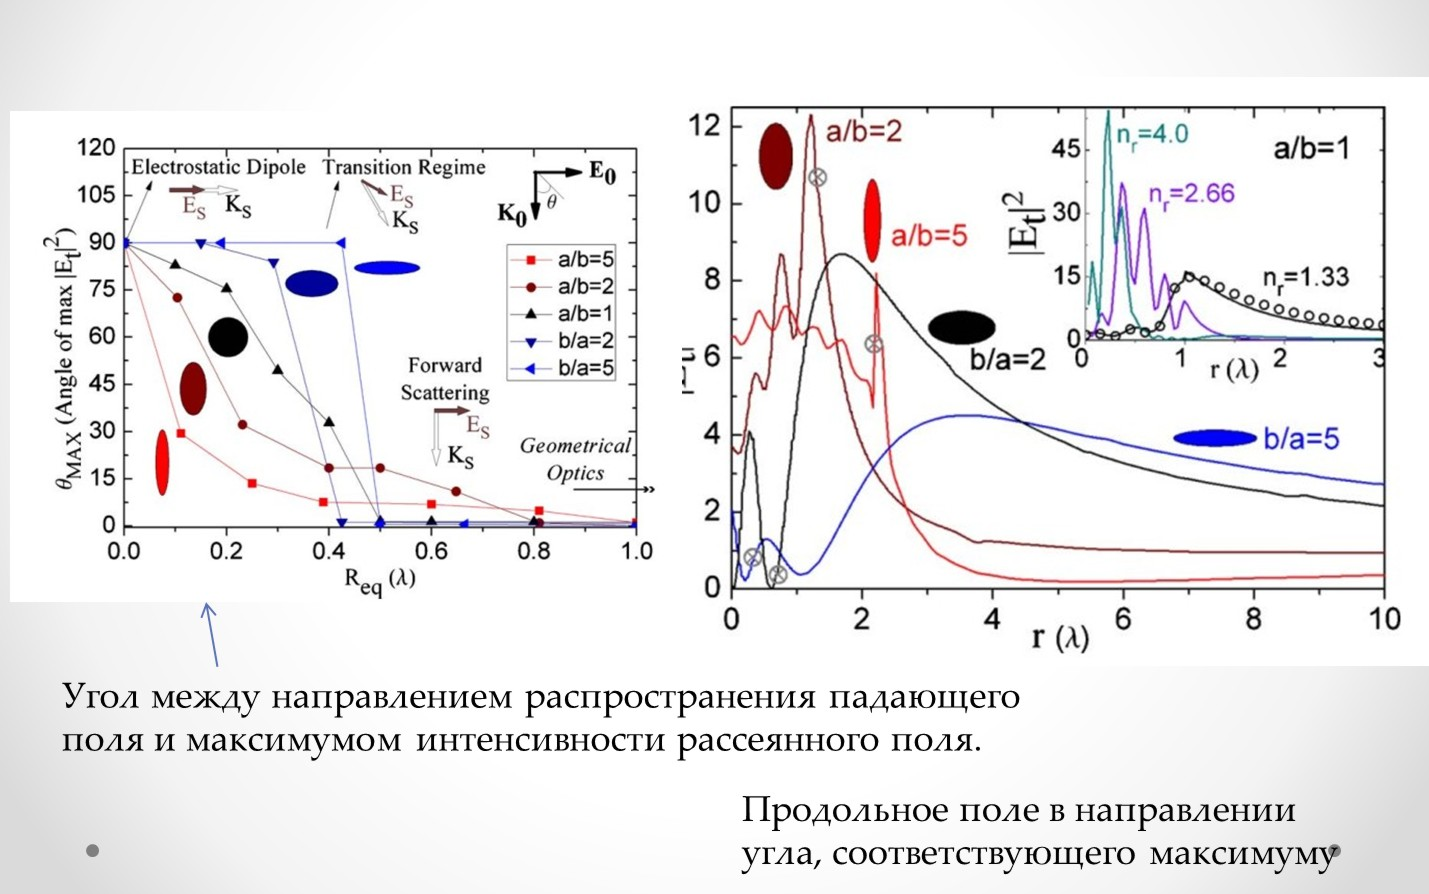
\includegraphics[width=1.1\textwidth]{add_sl4}
\end{center}

\end{frame}

\begin{frame}{Обобщение теории рассеяния Ми на эллипсоидальные формы (Ми-Ганса)}

\begin{center}
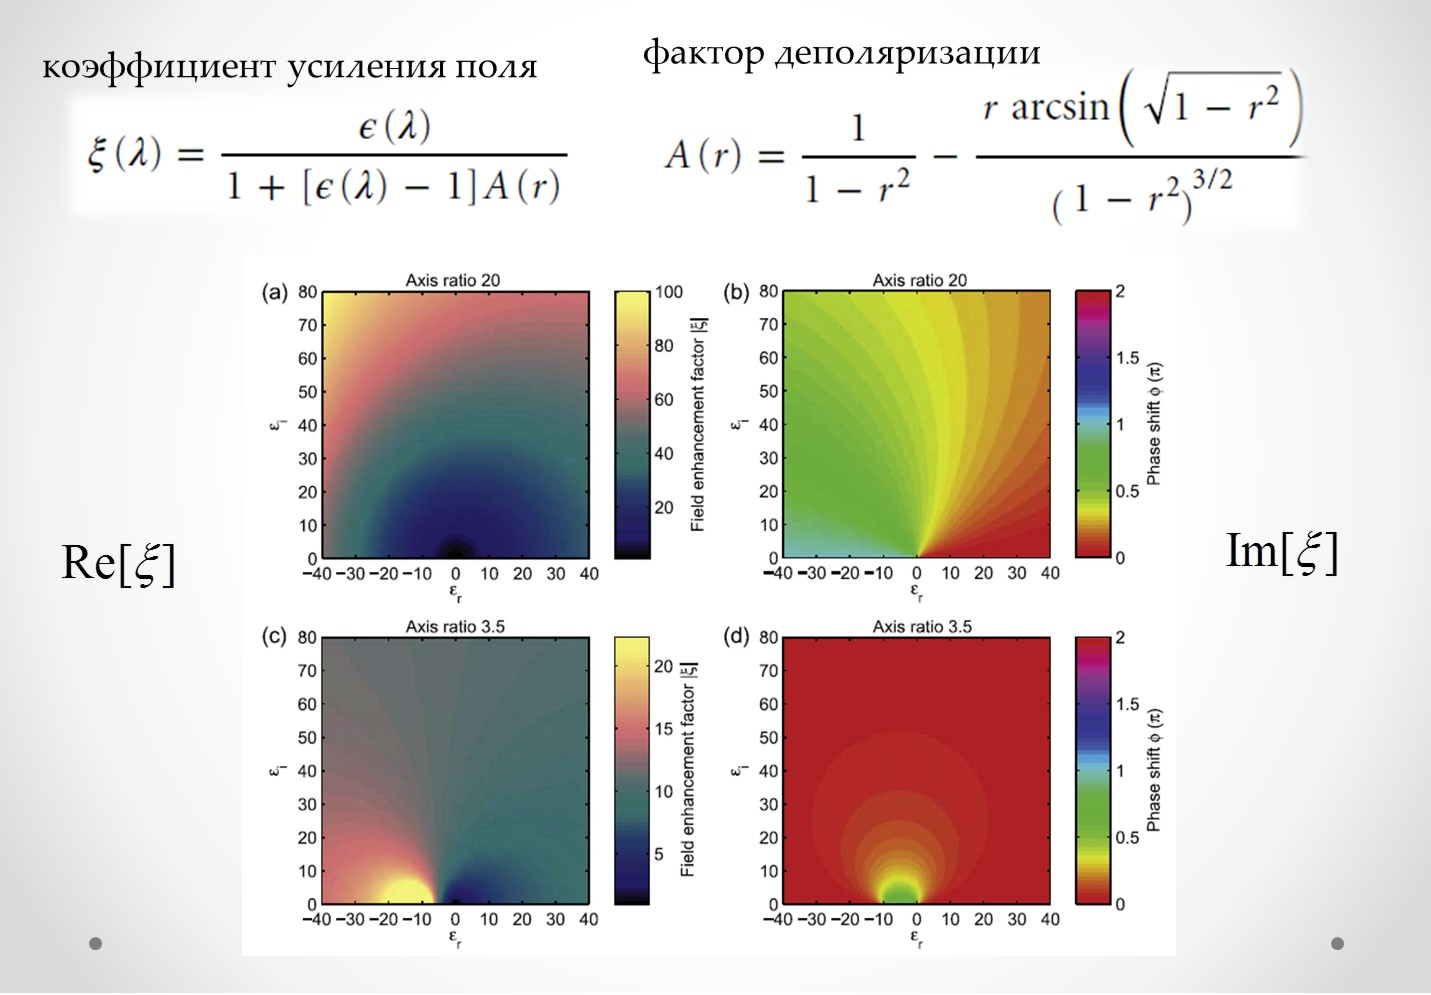
\includegraphics[width=1.1\textwidth]{add_sl5}
\end{center}
  
\end{frame}

\begin{frame}{Обобщение теории рассеяния Ми на эллипсоидальные формы (Ми-Ганса)}

\begin{center}
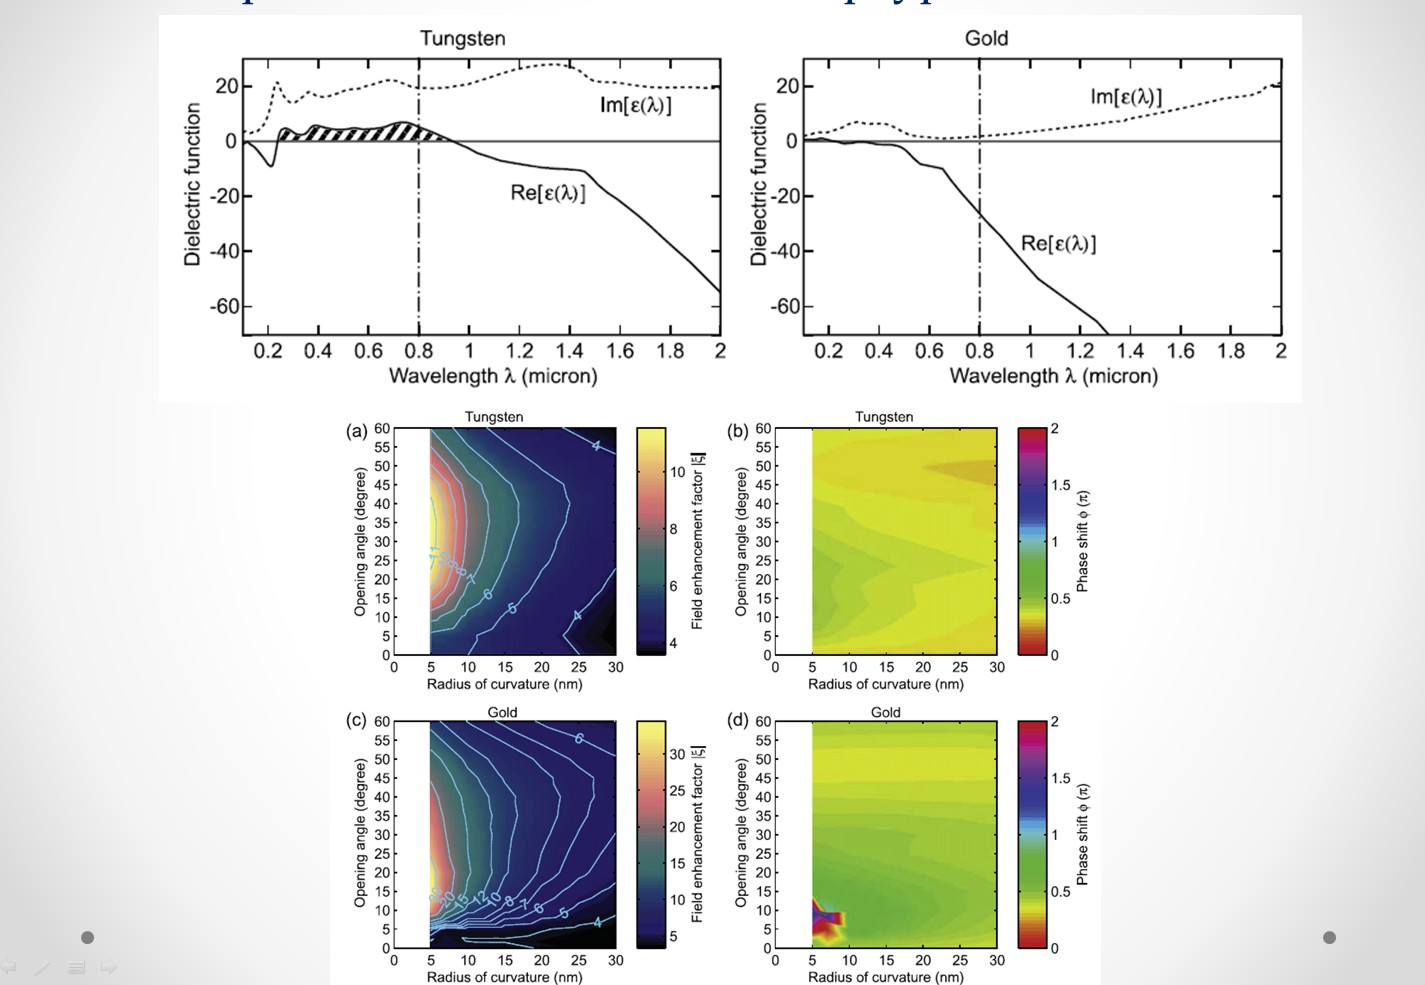
\includegraphics[width=1.1\textwidth]{add_sl6}
\end{center}

\end{frame}

\begin{frame}{Обобщение теории рассеяния Ми на эллипсоидальные формы (Ми-Ганса)}

\begin{center}
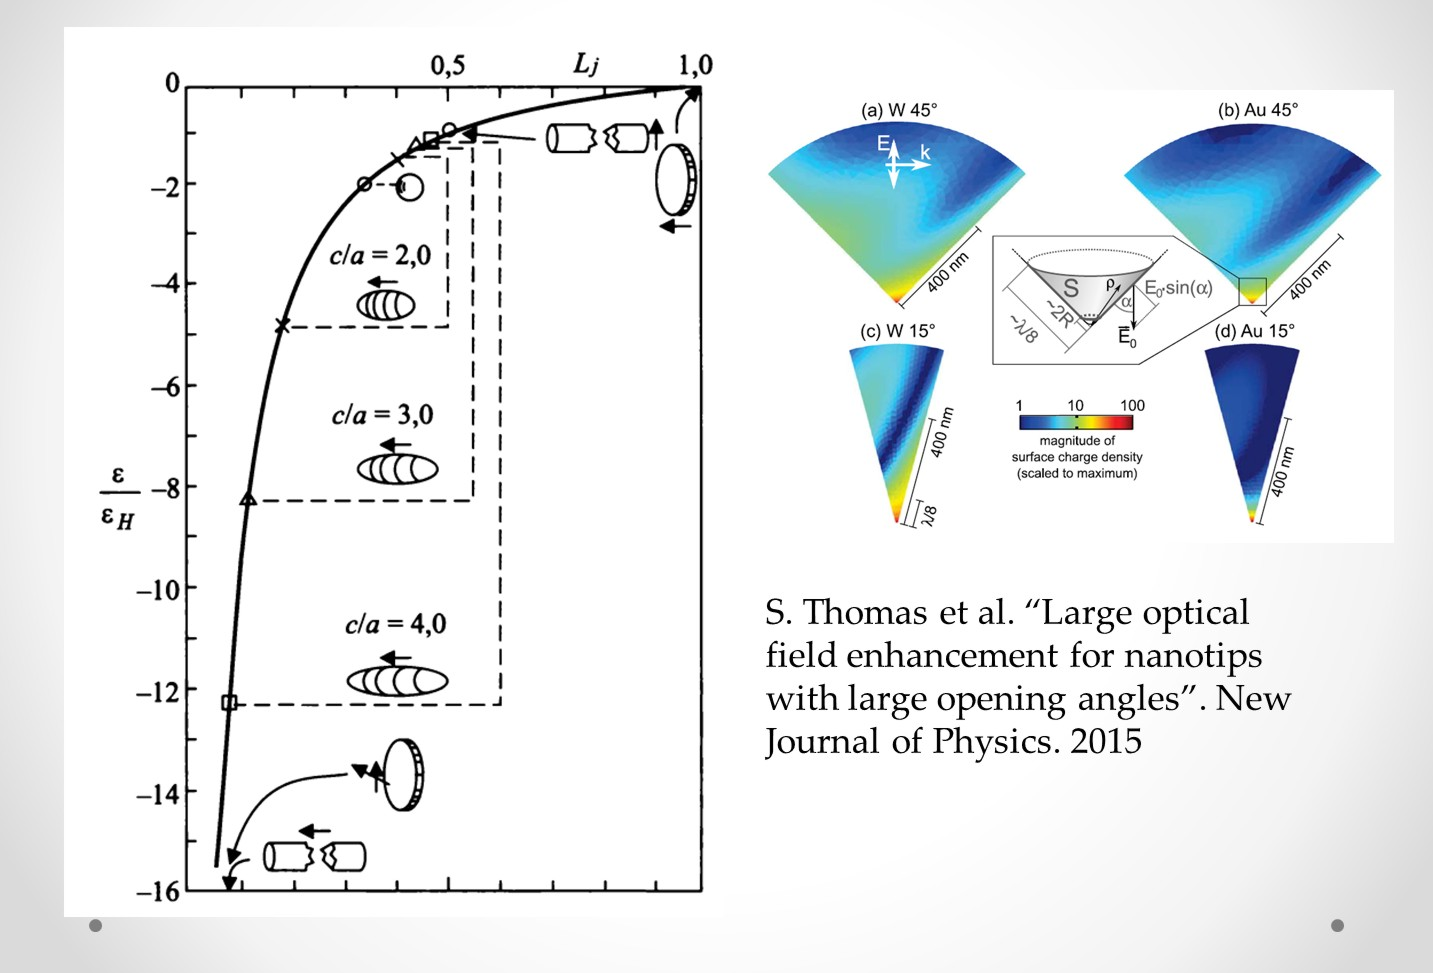
\includegraphics[width=1.1\textwidth]{add_sl7}
\end{center}
    
\end{frame}


\begin{frame}{Линейная ближнепольная микроскопия-I}

\begin{columns}[c]
\column{6.5cm}
\begin{center}
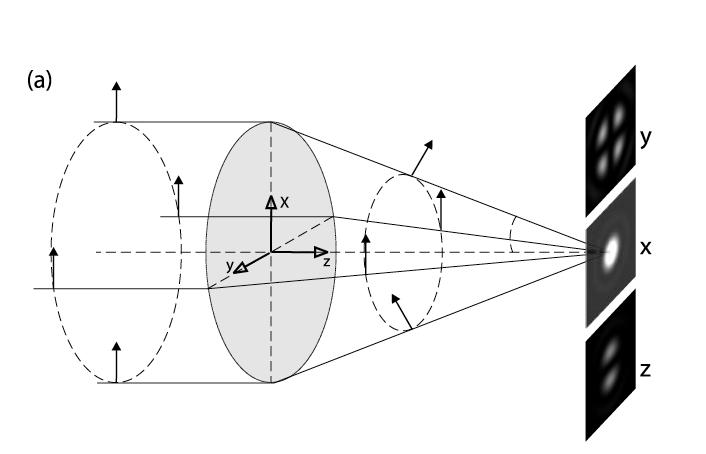
\includegraphics[width=0.9\textwidth]{sm0}
\end{center}

\column{6.5cm}
\begin{center}
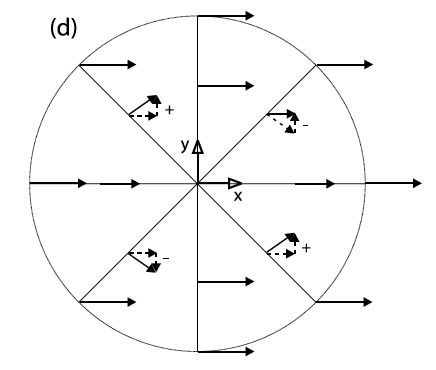
\includegraphics[width=0.9\textwidth]{sm1}
\end{center}
\end{columns}
\end{frame}

\begin{frame}{Линейная ближнепольная микроскопия-I}
\begin{columns}[c]
\column{6.5cm}
\begin{center}
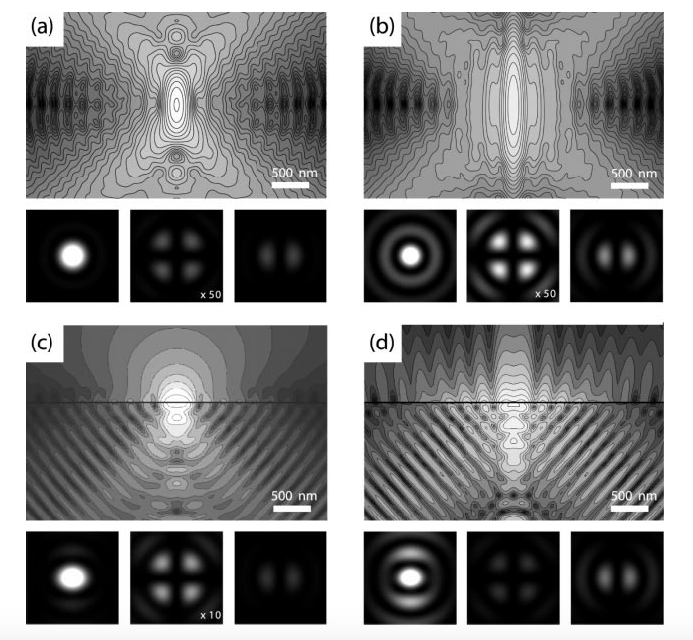
\includegraphics[width=0.9\textwidth]{sm2}
\end{center}

\column{6.5cm}
\begin{center}
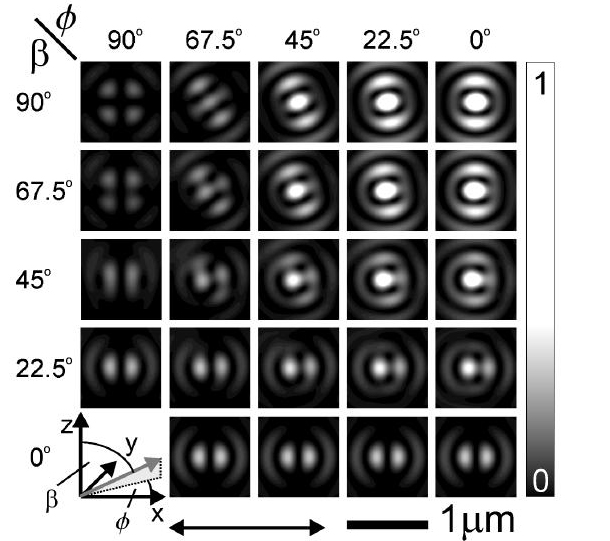
\includegraphics[width=0.9\textwidth]{sm3}
\end{center}


\end{columns}

\end{frame}

\begin{frame}{Линейная ближнепольная микроскопия-II}
\begin{columns}[c]
\column{6.5cm}
\begin{center}
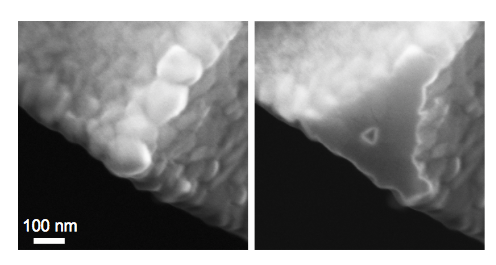
\includegraphics[width=0.9\textwidth]{tr7}
\end{center}

\column{6.5cm}
\begin{center}
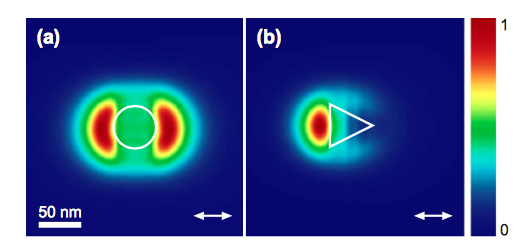
\includegraphics[width=0.9\textwidth]{tr6}
\end{center}

\end{columns}

"Обострение" геометрии ведет к большей локализации поля.

D. Molenda, G. Colas des Francs, U.C. Fischer, N. Rau, and A. Naber "High-resolution mapping of the optical near-field components at a triangular nano-aperture", OPTICS EXPRESS, 2005

\end{frame}

\begin{frame}{Линейная ближнепольная микроскопия-II}
\begin{columns}[c]
\column{6.5cm}
\begin{center}
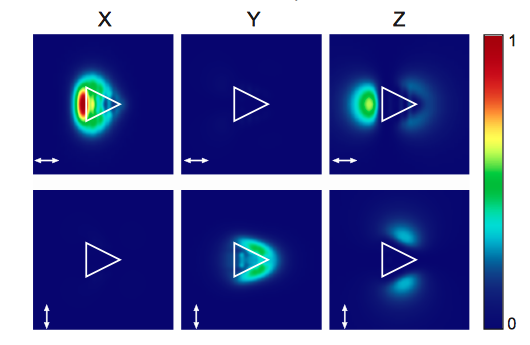
\includegraphics[width=0.9\textwidth]{tr3}
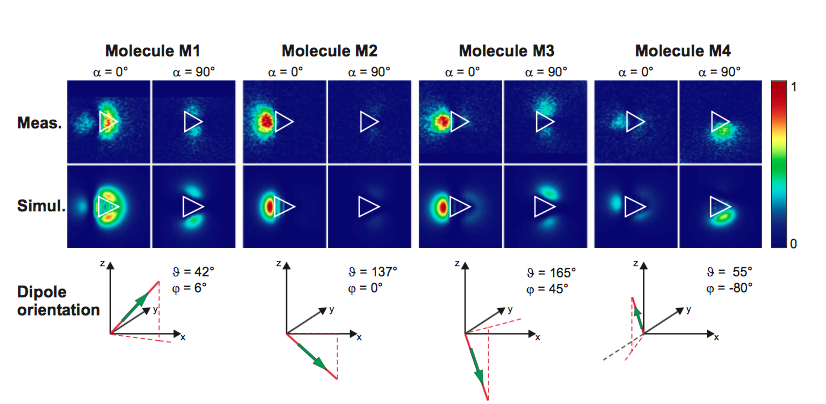
\includegraphics[width=0.9\textwidth]{tr2}
\end{center}

\column{6.5cm}
\begin{center}
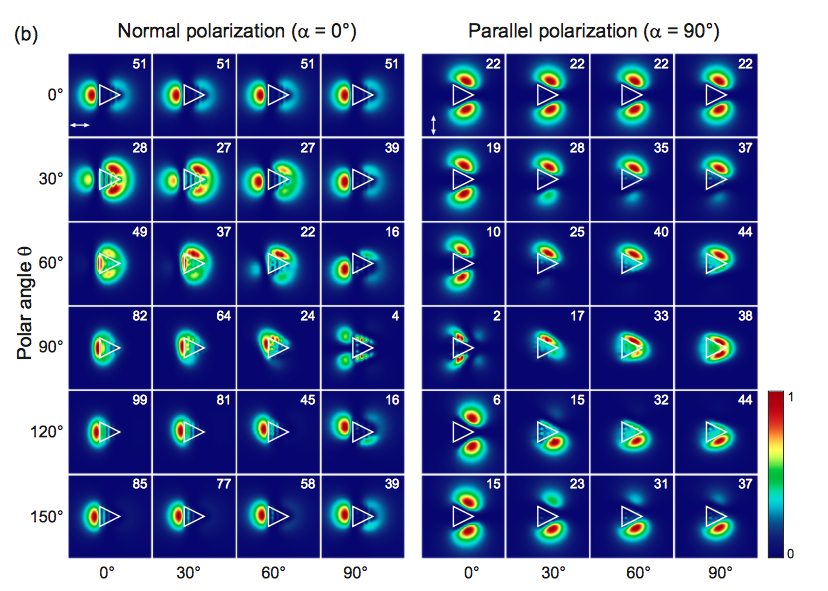
\includegraphics[width=0.9\textwidth]{tr4}
\end{center}


\end{columns}

\end{frame}

\begin{frame}{Линейная ближнепольная микроскопия-II}

\begin{center}
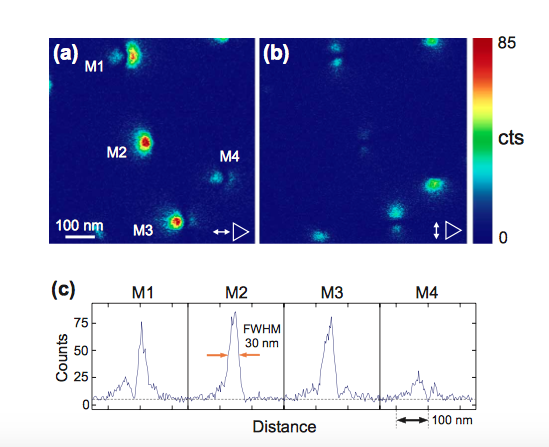
\includegraphics[width=0.9\textwidth]{tr5}
\end{center}


\end{frame}

\begin{frame}{Нелинейная ближнепольная микроскопия}

    
\begin{columns}[c]
\column{6.5cm}

Определение хиральности вещества при помощи генерации второй гармоники, возбуждаемой полем в гибридном состоянии поляризации.

\begin{center}
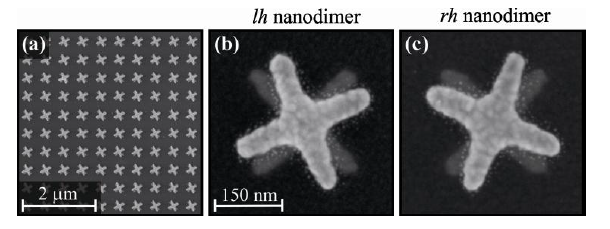
\includegraphics[width=\textwidth]{nanodimer1}
\end{center}

На примере в разные стороны закрученных нанодимеров (M. Hattunen et al. Nonlinear chiral imaging of subwavelength-sized twisted-cross nanodimers. 2011).
 
\column{6cm}
\begin{center}
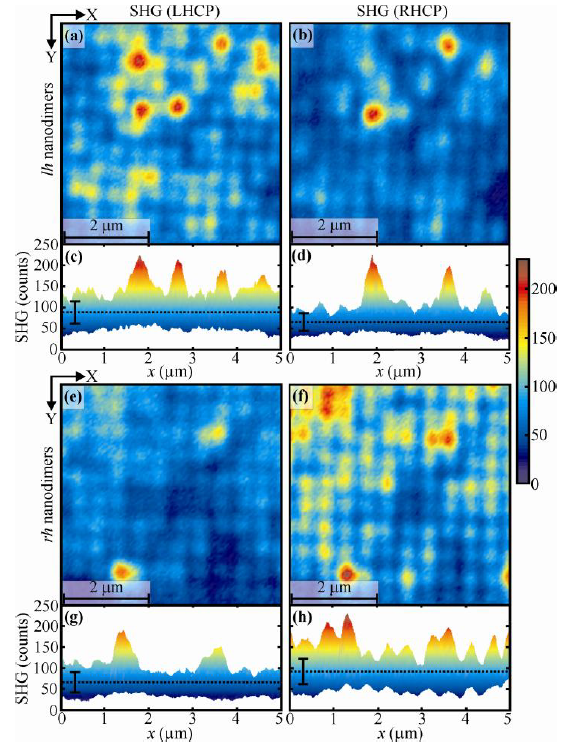
\includegraphics[width=0.85\textwidth]{nanodimer2}
\end{center}


\end{columns}
    
\end{frame}

\end{document}